\section{Visualisierung}

Da zum Zeitpunkt der Dokumentationserstellung keine reale Anlage zur Verfügung stand, wurde mit der SIMATIC HMI eine Visualisierung angefertigt (\autoref{fig:Bild3.1}). Die Visualisierung spiegelt den realen Aufbau wieder. Zur Überprüfung der Schütze (K3, K4), wurden zwei weitere Leuchtmelder eingefügt. Diese sind in der realen Anlage nicht vorhanden. Im Gegensatz zur realen Anlage können durch die Visualisierung nicht alle Sachverhalte korrekt dargestellt werden. Somit sind die Öffner-Taster mit dem Kommentar \glqq Toggle\grqq\:versehen, da in der Simulation keine öffnenden Taster eingefügt werden können. Bei der Bedienung ist darauf zu achten, dass ein Klicken das jeweilige Bit nur invertiert! Die Endlagentaster des Förderbands und der Förderschnecke sind durch B1 und B2 dargestellt und ebenfalls mit einem Kommentar versehen worden. 

\begin{figure}[H]
   \centering
   \fbox{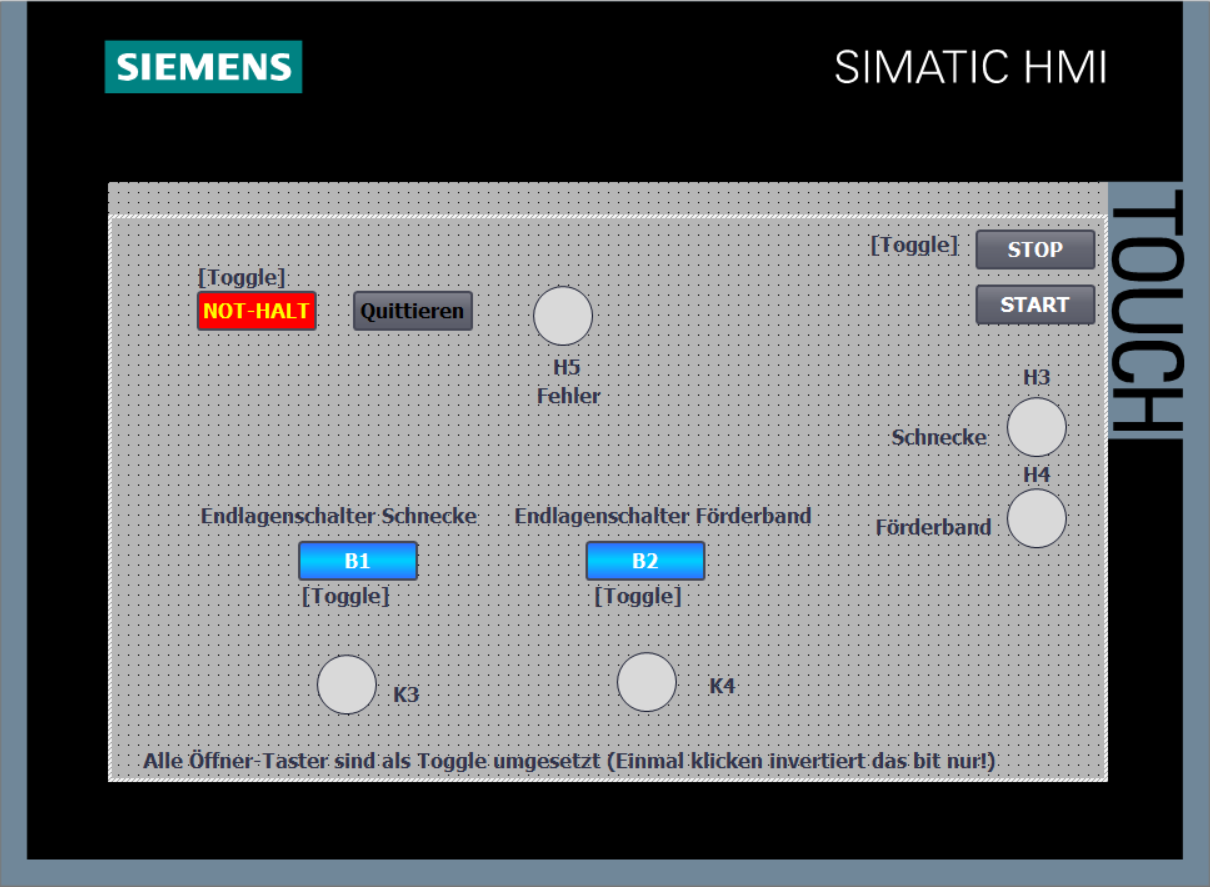
\includegraphics[width=0.8\textwidth]{Bilder/3. Visualisierung/Visualisierung_HMI.png}}
   \caption[Visualisierung mit SIMATIC HMI]{Visualisierung mit SIMATIC HMI unter Nutzung der Software WinCC}
   \label{fig:Bild3.1}
\end{figure}